\chapter{Desenhos de Negócios}


You can draw a triangle by trial and error, as I did to find the best point for putting the top edge in \autoref{fig:3angulo}, with single command \verb|\draw|, as shown in the following code.

\begin{verbatim}
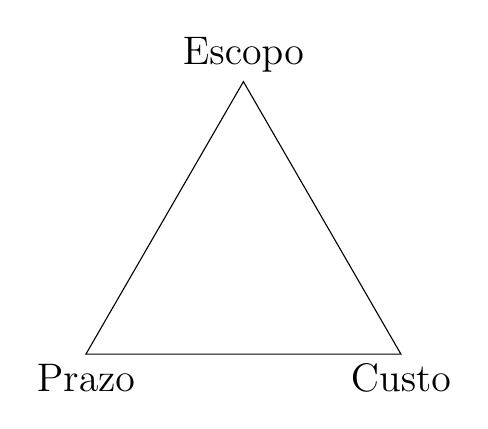
\begin{tikzpicture}
  \draw (-2,0) node[anchor=north]{\Large Prazo}   -- (2,0) node[anchor=north]{\Large Custo}  -- (0,3.46) node[anchor=south] {\Large Escopo}   -- cycle;
\end{tikzpicture}    
\end{verbatim}

\begin{figure}[hbt]
    \centering
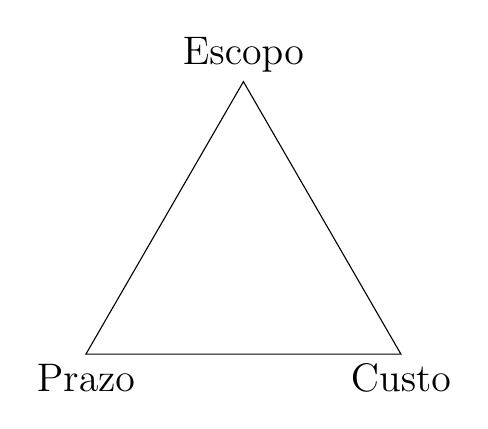
\begin{tikzpicture}
  \draw (-2,0) node[anchor=north]{\Large Prazo}   -- (2,0) node[anchor=north]{\Large Custo}  -- (0,3.46) node[anchor=south] {\Large Escopo}   -- cycle;
\end{tikzpicture}
    \caption{Triangle}
    \label{fig:3angulo}
\end{figure}

Another figure done by deciding where the edges should be \textit{a priori}, resulting in \autoref{fig:pyramid}. In this code, there is a good example of using \verb|foreach| to achieve a result. Also, the use of \verb|intersections| to calculate where a point is.

\begin{verbatim}
\begin{tikzpicture}

\coordinate (A) at (-3.5,0) {};
\coordinate (B) at ( 3.5,0) {};
\coordinate (C) at (0,6) {};

\path[name path=AC,draw=none] (A) -- (C);
\path[name path=BC,draw=none] (B) -- (C);

\filldraw[draw=black, ultra thick,fill=white] 
(A) -- (B) -- (C) -- cycle ;

\foreach \y/\A in {0/Despejo Controlado,
                   1/Aterro ou Incineração,
                   2/Reciclagem,
                   3/Reuso,
                   4/\parbox{3cm}{\centering
                   Redução}} 
    {
    \path[draw=none, very thick, dashed, name
    path=horiz] (A|-0,\y) -- (B|-0,\y);
    \draw[draw=black, very thick, dashed, 
          name intersections={of=AC and horiz,by=P},
          name intersections={of=BC and horiz,by=Q}]
          (P) -- (Q)
          node[midway,above,font=\bfseries\scshape,
          color=black] {\A};
}

\node[single arrow,rotate=90,draw=black,minimum
height=6cm] at (-4,3) {melhor opção};

\end{tikzpicture}    
\end{verbatim}


\begin{figure}[hbt]
\centering
\begin{tikzpicture}

\coordinate (A) at (-3.5,0) {};
\coordinate (B) at ( 3.5,0) {};
\coordinate (C) at (0,6) {};

\path[name path=AC,draw=none] (A) -- (C);
\path[name path=BC,draw=none] (B) -- (C);

\filldraw[draw=black, ultra thick,fill=white] (A) -- (B) -- (C) -- cycle ;

\foreach \y/\A in {0/Despejo Controlado,
                   1/Aterro ou Incineração,
                   2/Reciclagem,
                   3/Reuso,
                   4/\parbox{3cm}{\centering Redução}} 
    {
    \path[draw=none, very thick, dashed, name path=horiz] (A|-0,\y) -- (B|-0,\y);
    \draw[draw=black, very thick, dashed, 
          name intersections={of=AC and horiz,by=P},
          name intersections={of=BC and horiz,by=Q}] (P) -- (Q)
          node[midway,above,font=\bfseries\scshape,color=black] {\A};
}

\node[single arrow,rotate=90,draw=black,minimum height=6cm] at (-4,3) {melhor opção};

\end{tikzpicture}
\caption{A tipical pyramid of concepts.}
\label{fig:pyramid}
\end{figure}
